%%%%%%%%%%%%%%%%%%%%%%%%%%%%%%%%%%%%%%%%%%%%%%%%%%%%%%%%%%%%%%%%%%%%%%%%
% Plantilla TFG/TFM
% Universidad de A Coruña. Facultad de Informática
% Realizado por: Welton Vieira dos Santos
% Modificado: Welton Vieira dos Santos
% Contacto: welton.dossantos@udc.es
%%%%%%%%%%%%%%%%%%%%%%%%%%%%%%%%%%%%%%%%%%%%%%%%%%%%%%%%%%%%%%%%%%%%%%%%


\chapter{Análisis de Viabilidad: Modelado de la Organización.}

\newpage
\section{Formulario OM-1: Contexto Organizacional, problemas y soluciones.}
Identificación de los problemas y oportunidades orientadas al conocimiento de la organización, como se muestra en la Tabla \ref{tab:OM1}.


\begin{table}[H]
\scriptsize
\begin{tabularx}{\textwidth}{|l|X|} \hline
\textbf{Modelo de Organización} & \textbf{Formulario OM-1: Problemas y Posibilidades de Mejora} \\ \hline\hline

\textsc{Problemas y Oportunidades} & Invertir o especular con activos financieros en bolsa de valores es una labor bastante compleja, ya que si una persona no tiene el conocimiento suficiente y adecuado puede ser un auténtico ``desastre''. Con ese panorama, se presenta una oportunidad para desarrollar sistemas que sean capaces de hacer esa labor con el menor error posible y con ganancias muy superior a media de operaciones hechas actualmente en el mercado financiero. Además de acercar esa práctica de inversión a particulares (conocidos como inversores minoritarios), que generalmente no tiene mucho capital para hacer inversiones mas seguras.\\ \hline
\textsc{Contexto Organizacional} & 
\begin{enumerate}
  \item La Misión, visión y objetivos de la organización son:  
  \begin{enumerate}
    \item \textbf{Misión:} Una pequeña empresa (Startup) de desarrollo de aplicaciones inteligentes relacionadas con el mercado financiero.
    \item \textbf{Visión:} Dando continuidad de un sistema inteligente desarrollado anteriormente, donde el sistema sólo lidiaba con mercados de acciones y ahora funcionará con los mercados de divisas (Forex).
    \item \textbf{Objetivos:} Seguir creciendo como empresa desarrolladora y seguir expandiendo las ventas de nuestras soluciones inteligentes para que en el futuro se pueda comercializar de forma globalizada.
  \end{enumerate}
  \item Estrategia de organización: desenvolver un producto de sofware con un coste accesible para que tenga un gran público.
  \item Escala de valores por la que se rige: obtener el máximo benefício que el mercado financiero pueda ofrecer.
\end{enumerate}    \\ \hline
\textsc{Soluciones} & La solución que se propone es desarrollar un sistema bajo coste que sea eficaz y eficiente para que un inversor minorista pueda especular en los mercados de divisa (Forex) de una forma segura y con unos beneficios razonables con respecto al riesgo del capital invertido. \\
\hline
\end{tabularx}
  %\label{tab.OM1}
  \caption{\label{tab:OM1}Contexto Organizacional - OM1}
\end{table}
	
 
%%%%%%%%%%%%%%%%%%%%%%%%%%%%%%%%%%%%%%%%%%%%%%%%%%%%%%%%%%%%%%%%%%%%%%%%%%%%%%%
\section{Formulario OM-2: descripción del área de interés de la organización.}

Descripción de los aspectos de la organización que tienen impacto y/o se ven afectados
  por las soluciones basadas en conocimiento elegidas.


\begin{table}[H]
\scriptsize
\begin{tabularx}{\textwidth}{|l|X|} \hline
\textbf{Modelo de Organización} & \textbf{Formulario OM-2: Aspectos Variables} \\ \hline\hline

\textsc{Estructura} & Se presenta un gráfico de la parte de la organización (Figura \ref{fig:diagramaEstructura}) bajo análisis en términos de departamentos, grupos, unidades\dots\\ \hline

\textsc{Procesos} & Abrir operativas en el mercado de Forex\\ \hline
\textsc{Personal} &  Todos los miembros de nuestra Startup está composto por profesionales altamente cualificados, todos trabajan en cada parte del proyecto utilizando una metodologia Scrum.\\ \hline
\textsc{Recursos} &  Describir los recursos utilizados por los procesos:
\begin{enumerate}
    \item Sistemas de información y otros recursos computacionales:
    \begin{enumerate}
      \item Sistema inteligente de predicción
      \item Sistema de apertura de operativa en el mercado.
      \item Base de datos de mercado Forex.
      \item Apoyo de herramientas de lectura de mercado
    \end{enumerate}
    \item Equipamiento y material.
    \begin{enumerate}
      \item Sistema informático
      \item Conexión a Internet.
      \item Servidor de conexión con el mercado financiero.
    \end{enumerate}
\end{enumerate}
\\ \hline
\textsc{Conocimiento} &  Un experto/s en especulación en mercado de divisas.\\ \hline
\textsc{Cultura y Potencial} &  Todos los miembros tiene la misma responsabilidad dentro del proyecto. La comunicación, cordialidad y el respecto mutuo es la tónica más importante para el desarrollo del proyecto.\\ \hline
\end{tabularx}
  %\label{tab.OM2}
  \caption{\label{tab:OM2}Descripción del área de interés de la organización - OM2}
\end{table}
\begin{figure}[H]
	\centering
	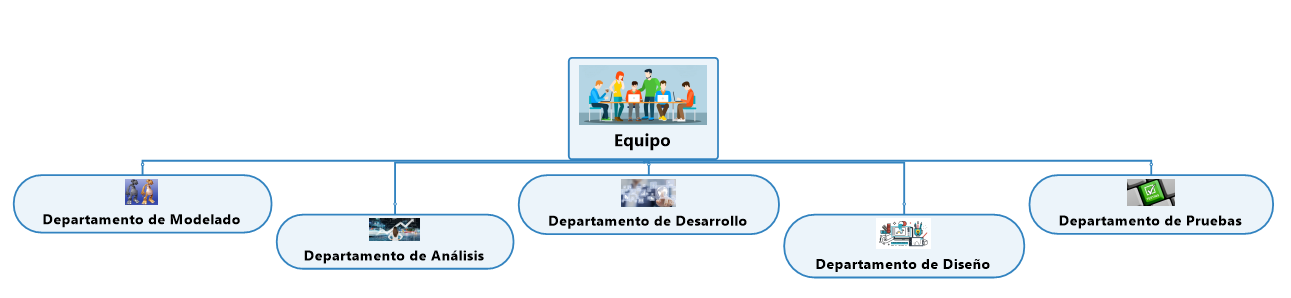
\includegraphics[scale=0.40]{imaxes/diagramaEstructura_2.png}
	\caption{\label{fig:diagramaEstructura}Diagrama estructura - Formulario OM2}
\end{figure}

\section{Formulario OM-3: Descomposición del Proceso de Negocio.}

Descripción del proceso de interés a partir de las tareas que lo componen.

\begin{table}[H]
  \centering
  \resizebox{18,0cm}{!}{
    \begin{tabular}{|c|c|c|c|c|c|c|}
      \hline
      \multicolumn{3}{|c}{\textbf{Modelo de Organización}} & \multicolumn{4}{|c|}{\textbf{Formulario OM-3: Descomposición de los Procesos}}\\
      \hline \hline
      \textsc{N\textordmasculine} & \textsc{Tarea} & \textsc{Realiza\-da por} & \textsc{¿Dónde?} & \textsc{Recursos de Conocimiento} & \textsc {¿In\-ten\-si\-va en Conocimiento?} & \textsc{Im\-por\-tan\-cia} \\
      \hline

      1 & Análisis de mercado & \multicolumn{1}{|p{6.0cm}|}{\centering Inversor (usuario)}& \multicolumn{1}{|p{5.0cm}|}{\centering En PC del inversor (usuario)} & \multicolumn{1}{|p{6.0cm}|}{\centering Experiencia en especulación de activos financieros y teorías de análisis de mercado (La Metodología Wyckoff en Profundidad - \textit{Rubén Villahermosa})} & Sí (elevado) & Alta \\
      \hline
      2 & Introducir datos gestión & \multicolumn{1}{|p{6.0cm}|}{\centering Inversor (usuario)} & \multicolumn{1}{|p{5.0cm}|}{\centering En el PC del inversor (usuario)} & \multicolumn{1}{|p{6.0cm}|}{\centering Experiencia de gestión por parte del inversor (usuario)} & Sí (moderado) & Alta \\
      \hline
      3 & Operación Comprar & \multicolumn{1}{|p{6.0cm}|}{\centering Inversor (usuario )}& \multicolumn{1}{|p{5.0cm}|}{\centering En PC del inversor (usuario)} & \multicolumn{1}{|p{6.0cm}|}{\centering Experiencia en compra de activos en mercado de divisas} & Sí (elevado) & Máxima \\
      \hline
      4 & Operación vender & \multicolumn{1}{|p{6.0cm}|}{\centering Inversor (usuario)}& \multicolumn{1}{|p{5.0cm}|}{\centering En PC del inversor (usuario)} & \multicolumn{1}{|p{6.0cm}|}{\centering Experiencia en venta de activos en mercado de divisas} & Sí (elevado) & Máxima \\
      \hline      
      5 & \multicolumn{1}{|p{6.0cm}|}{\centering Gestionar las operativas abiertas} & \multicolumn{1}{|p{6.0cm}|}{\centering Inversor (usuario)} &  \multicolumn{1}{|p{5.0cm}|}{\centering En PC del inversor (usuario)} & \multicolumn{1}{|p{6.0cm}|}{\centering Experiencia en gestionar las operativas de compra y venta de activos al mercado de divisas. Teorías de gestión de capital de inversión} & Sí (elevado) & Máxima \\
      \hline
    \end{tabular}
  }
	\caption{\label{tab:OM3}Descomposición del proceso de negocio - OM3}
\end{table}

\newpage
\section{Formulario OM-4: Activos de Conocimiento}
%%%%%%%%%%%%%%%%%%%%%%%%%%%%%%%%%%%%%%%%%%%%%%%%%%%%%%%%%%%%%%%%%%%%%%%%%%%%%%%

Descripción del componente \textit{conocimiento} del modelo de la organización.

\begin{table}[H]
  \centering
  \resizebox{15,0cm}{!}{
    \begin{tabular}{|c|c|c|c|c|c|c|}
      \hline
      \multicolumn{3}{|c}{\textbf{Modelo de Organización}} & \multicolumn{4}{|c|}{\textbf{Formulario OM-4: Activos de Conocimiento}}\\
      \hline \hline
      \textsc{Recurso de Conocimiento} & \textsc{Pertenece} & \textsc{Usado en} & \textsc{¿Forma Cor\-recta?} & \textsc{¿Lugar Cor\-recto?} & \textsc {¿Tiempo Cor\-recto?} & \textsc{¿Calidad Cor\-recta?} \\
      \hline
      \multicolumn{1}{|p{6.0cm}|}{\centering Experiencia en especulación de activos financieros} & \multicolumn{1}{|p{6.0cm}|}{\centering Expertos en especulación en mercados de activos} & \multicolumn{1}{|p{6.0cm}|}{\centering Tarea 1 de OM-3} & \multicolumn{1}{|p{6.0cm}|}{\centering No, el conocimiento reside en experiencia del experto (inversor).} & Departamento de Análisis & - & \multicolumn{1}{|p{6.0cm}|}{\centering Sí, teniendo en cuenta que son aproximaciones.} \\      
      \hline
      \multicolumn{1}{|p{6.0cm}|}{\centering Teorías de análisis de mercado (La Metodología Wyckoff en Profundidad - \textit{Rubén Villahermosa})} & \multicolumn{1}{|p{6.0cm}|}{\centering Expertos en especulación en mercados de activos} & \multicolumn{1}{|p{6.0cm}|}{\centering Tarea 1 de OM-3} & \multicolumn{1}{|p{6.0cm}|}{\centering Si, Utilizar la teoría de identificación de tendencias de mercado, identificar los soportes y resistencias dejado por la oscilación del precio al largo del tiempo} & Departamento de Análisis & - & \multicolumn{1}{|p{6.0cm}|}{\centering Sí, teniendo en cuenta que son aproximaciones} \\      
      \hline 
      \multicolumn{1}{|p{6.0cm}|}{\centering Experiencia de gestión por parte del inversor (usuario)} & \multicolumn{1}{|p{6.0cm}|}{\centering Expertos en especulación en mercados de activos} & \multicolumn{1}{|p{6.0cm}|}{\centering Tarea 2 de OM-3} & \multicolumn{1}{|p{6.0cm}|}{\centering No, el conocimiento reside en el experto (inversor)} &  Departamento de Análisis  & - & \multicolumn{1}{|p{6.0cm}|}{\centering Sí, teniendo en cuenta que son aproximaciones.} \\
      \hline
      \multicolumn{1}{|p{6.0cm}|}{\centering Experiencia en compra de activos en mercado de divisas.} & \multicolumn{1}{|p{6.0cm}|}{\centering Expertos en especulación en mercados de activos} & \multicolumn{1}{|p{6.0cm}|}{\centering Tarea 3 de OM-3} & \multicolumn{1}{|p{6.0cm}|}{\centering No, el conocimiento reside en el experto (inversor)} &  Departamento de Análisis  & - & \multicolumn{1}{|p{6.0cm}|}{\centering Sí, teniendo en cuenta que son aproximaciones} \\
      \hline
      \multicolumn{1}{|p{6.0cm}|}{\centering Experiencia en venta de activos en mercado de divisas} & \multicolumn{1}{|p{6.0cm}|}{\centering Expertos en especulación en mercados de activos} & \multicolumn{1}{|p{6.0cm}|}{\centering Tarea 4 de OM-3} & \multicolumn{1}{|p{6.0cm}|}{\centering No, el conocimiento reside en el experto (inversor)} &  Departamento de Análisis  & - & \multicolumn{1}{|p{6.0cm}|}{\centering Sí, teniendo en cuenta que son aproximaciones} \\
      \hline
      \multicolumn{1}{|p{6.0cm}|}{\centering Experiencia en gestionar las operativas de compra y venta de activos al mercado de divisas} & \multicolumn{1}{|p{6.0cm}|}{\centering Expertos en especulación en mercados de activos} & \multicolumn{1}{|p{6.0cm}|}{\centering Tareas 5 de OM-3} & \multicolumn{1}{|p{6.0cm}|}{\centering No, el conocimiento reside en el experto (inversor)} &  Departamento de Análisis  & - & \multicolumn{1}{|p{6.0cm}|}{\centering Sí, teniendo en cuenta que son aproximaciones} \\
      \hline
      \multicolumn{1}{|p{6.0cm}|}{\centering Teorías de gestión de capital de inversión} & \multicolumn{1}{|p{6.0cm}|}{\centering Expertos en especulación en mercados de activos} & \multicolumn{1}{|p{6.0cm}|}{\centering Tareas 5 de OM-3} & \multicolumn{1}{|p{6.0cm}|}{\centering Si, utilizar los mecanismos de reducción de riesgos y frenado de pérdidas} &  Departamento de Análisis  & - & \multicolumn{1}{|p{6.0cm}|}{\centering Sí, pero depende muchísimo del mercado.} \\
      \hline
    \end{tabular}
  }
	\caption{\label{tab:OM4}Activos de conocimiento - OM4}
\end{table}

\clearpage